\section{$\text{H}_2$/$\text{O}_2$ reaction kinetics: higher-dimensional case}
\label{sec:app}

For the high-dimensional case, we aim to investigate the impact of the uncertain
pre-exponents ($A_i$'s) as well as the activation energies ($E_{a,i}$'s) \rebut{and
the initial conditions: pressure~($P_0$), temperature~($T_0$), and stoichiometry based on
the equivalence ratio~($\Phi_0$)} on ignition delay during the H$_2$/O$_2$ reaction. 
\rebut{The $\log(A_i)$'s, $E_{a,i}$'s for all reactions except 
$\mathcal{R}_6$ -- $\mathcal{R}_9$, $\mathcal{R}_{13}$ (due to 
zero nominal values for $E_a$), and the initial conditions were perturbed by
<<<<<<< HEAD
2$\%$ about their nominal values. Note that the mangnitude of the perturbation
was selected such that the ignition delay assumes a physically meaningful
value in the input
=======
2$\%$ about their nominal values. Note that the magnitude of the perturbation
was selected such that the ignition delay remains positive throughout the input
>>>>>>> 4d4dbf7e7af6f08bff040b4aee5683f6638be4d6
domain. The nominal values of the rate parameters, $A_i$'s and $E_{a,i}$'s 
were taken from~\cite{Yetter:1991}. The nominal values of $P_0$, $T_0$, and
$\Phi_0$ were considered to be 1.0 atm, 900~K, and 2.0 respectively.}

\subsection{Computing the active subspace}

The active subspace was computed using the iterative procedure outlined in 
Algorithm~\ref{alg:grad}. The convergence of the eigenvectors was examined
by tracking the quantity `$\max(\delta \hat{\mat{W}}_{1,j}^{(i)})$'. 
\rebut{In Figure~\ref{fig:conv_app}~(right), we examine $\max(\delta \hat{\mat{W}}_{1,j}^{(i)})$
with increasing iterations for the perturbation and the regression approaches 
discussed earlier in Section~\ref{sec:method}}. 
%
\begin{figure}[htbp]
 \begin{center}
  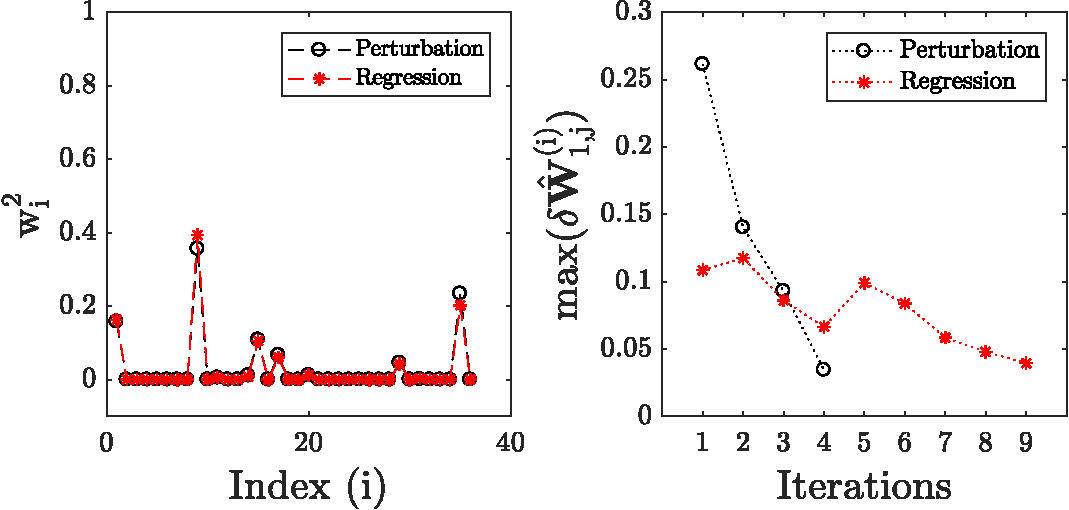
\includegraphics[width=0.8\textwidth]{./Figures/eig_conv36Dp2}
\caption{\rebut{Left: An illustrative comparison of individual components of the 
dominant eigenvector in the converged active subspace i.e., at the end
of 4 iterations in the perturbation approach and 9 iterations in the
regression approach. Right: A comparison of the convergence behavior
of the perturbation and the
regression approaches. Convergence is accomplished once 
$\max(\delta \hat{\mat{W}}_{1,j}^{(i)})$ assumes a value smaller
than 0.05.}}
\label{fig:conv_app}
\end{center}
\end{figure}
%
\rebut{At each iteration, we improve our estimates of the matrix $\hat{\mat{C}}$ by
estimating the gradient of the ignition delay at 5 new randomly generated samples 
in the 36-dimensional input space. However, gradient computation at these
5 samples requires 185 (=5$\times$(36+1)) model runs when using perturbation. 
For the same computational effort, the regression approach can afford 185 new
samples at each iteration. It is observed that using $\tau$ = 0.05, the 
active subspace requires 4 iterations (925 model runs) to converge in the case of perturbation, and
9 iterations (1850 model runs) to converge in the case of regression. Hence, the computational effort
required to obtain a converged active subspace is doubled when using
regression to approximate the gradient. Moreover, gradient estimation in the perturbation approach
can be made more efficient by using techniques such as automatic differentiation~\cite{Kiparissides:2009}
and adjoint computation~\cite{Jameson:1988}. These techniques although not pursued here are 
promising directions for
future efforts pertaining to this work. In Figure~\ref{fig:conv_app}~(right), we compare
individual components of the dominant eigenvector in the converged active subspace
obtained using the two approaches. The components are observed to be in excellent
agreement with each other.}

\rebut{In Figure~\ref{fig:hd}, we plot the SSP for the perturbation approach (left) and the regression
approach (center) in a 1-dimensional active subspace. A 1-dimensional polynomial fit is also
illustrated in both cases. Moreover, the two surrogates are shown to be consistent with each other (right).
From these results, it is clear that a 1-dimensional active subspace captures the variability in the
ignition delay with reasonable accuracy, and that the two approaches yield consistent results.}
%
\begin{figure}[htbp]
 \begin{center}
   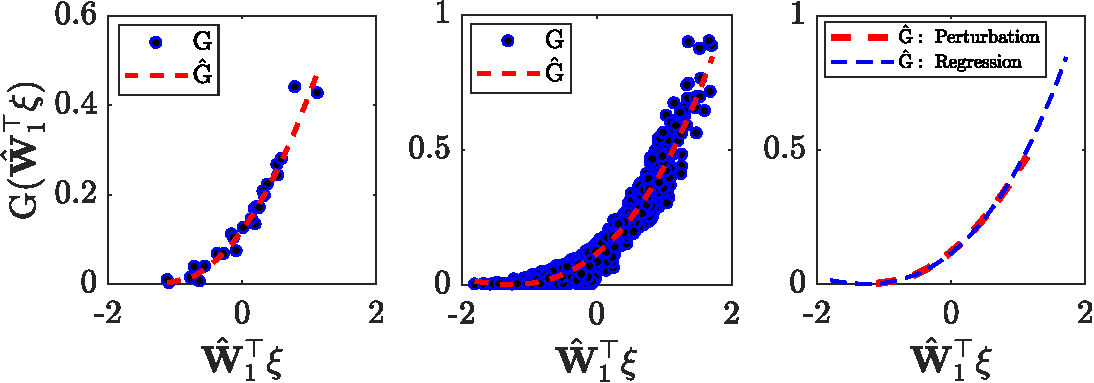
\includegraphics[width=0.9\textwidth]{./Figures/SSP_plot36Dp2}
\caption{\rebut{Sufficient summary plots (SSPs) for the case of perturbation (left) and regression (center).
A polynomial fit of degree 2 and 3 as shown in the plots is used as a surrogate in the 
perturbation and regression approaches respectively. An illustrative comparison of the two
surrogates is also provided (right).}}
\label{fig:hd}
\end{center}
\end{figure}
%

\subsection{Surrogate Assessment}
\label{sub:verify}

The 1-dimensional surrogate ($\hat{G}$) shown in Figure~\ref{fig:hd} is investigated
for its accuracy as well as the ability to capture the uncertainty in the
model output in two ways. Firstly, we estimate the relative L$^2$ norm of the discrepancy~($\varepsilon_d$)
between estimates of ignition delay in the case of H$_2$/O$_2$ reaction, obtained using the 
model output and the surrogate in the following equation:
%
\be
\varepsilon_d = \frac{\|G(\bm{\xi}) - \hat{G}(\bm{\xi})\|_2}{\|G(\bm{\xi})\|_2}
\ee
%
Model evaluations ($G$) at 10$^{4}$ random samples in the input domain were used to evaluate $\varepsilon_d$. 
\rebut{It was estimated to be approximately 0.17 for both approaches. Hence, the predictive accuracy of
the two approaches is comparable with respect to the relative L$^2$ norm of the discrepancy.
 However, as mentioned earlier, the computational effort required for
obtaining a converged active subspace using perturbation was half of that required when using
regression to estimate the model gradient at random samples in the 36-dimensional input domain.}

Secondly, we verified the accuracy of the two surrogates in a probabilistic setting. In particular, we compared 
probability density functions (PDFs) obtained using the true set of model evaluations, and 1-dimensional
surrogates ($\hat{G}$'s) based on the two approaches for gradient estimation as shown in 
Figure~\ref{fig:pdf_36D}. Note that the three PDFs were evaluated using the same set of 10$^4$ samples in the 
cross-validation set. 
%
\begin{figure}[htbp]
\begin{center}
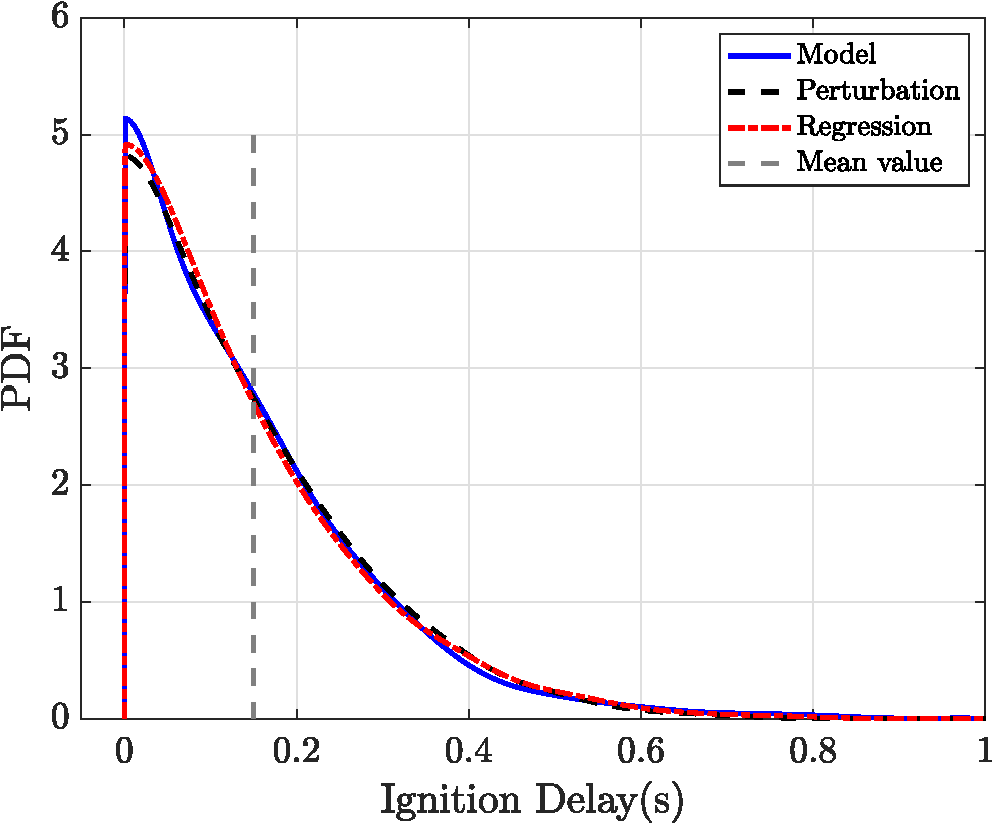
\includegraphics[width=3.0in]{./Figures/pdf_plot36Dp2}
\end{center} 
\caption{\rebut{A comparison of the PDFs of ignition delay, obtained using model 
evaluations (solid line) and 1-dimensional surrogates using the regression-based strategy (dashed line) and the
perturbation-based strategy (dashed-dotted line). The same set of 10$^4$ samples in the cross-validation set were 
used in each case.}}
\label{fig:pdf_36D}
\end{figure}
%
\rebut{The PDFs are observed to be in close agreement with each other. Specifically, the modal
estimate and the uncertainty (quantified by the spread in the distributions) is found to be consistent for the three 
cases. To confirm this, we compute the first-order (mean) and the second-order (standard deviation) statistics
of the estimates of the ignition delay obtained using the model, 1-dimensional surrogate from perturbation, and
1-dimensional surrogate from regression at the cross-validation sample set. The mean and standard deviation
estimates are provided in Table~\ref{tab:stats}.}
%
\begin{table}[htbp]
\begin{center}
\begin{tabular}{ccc}
\toprule
$\textbf{Distribution}$ & $\mu$ & $\sigma$ \\ 
\bottomrule
$G$~(Model) & \rebut{0.1510} & \rebut{0.1373} \\
$\hat{G}$~(Perturbation-based) & \rebut{0.1514} & \rebut{0.1275} \\
$\hat{G}$~(Regression-based) & \rebut{0.1510} & \rebut{0.1330} \\
\bottomrule
\end{tabular}
\caption{The mean ($\mu$), and the standard deviation ($\sigma$), computed using the model ($G$), and
the surrogate ($\hat{G}$) based on the two strategies at 10$^4$ samples in the cross-validation
set.}
\label{tab:stats}
\end{center}
\end{table}
%
\rebut{The mean and the standard deviation estimates obtained using the model and the 1-dimensional surrogates
are found to be in close agreement. It is interesting to note that estimates from the regression approach are
observed to be slightly more accurate. This is due to the fact that the converged active subspace in this case is 
based on 1850 samples in the 36-dimensional input domain, whereas, the converged active subspace based the 
perturbation approach is based on only 25 samples. As a result, the surrogate based on regression explores
a much wider range of values of the ignition delay compared to the surrogate based on perturbation as shown in
Figure~\ref{fig:hd}~(right).}

\subsection{GSA consistency check}

The normalized activity scores ($\tilde{\nu}_{i,r}$) based on the 1-dimensional active subspace, obtained
using the two approaches for gradient estimation (perturbation and regression),
are compared with the 
total-effect Sobol' indices
in Figure~\ref{fig:as_36D}. Note that the Sobol' indices were computed using the verified
1-dimensional surrogate ($\hat{G}$) in the active subspace, obtained using the 
perturbation approach. 
%
\begin{figure}[htbp]
 \begin{center}
  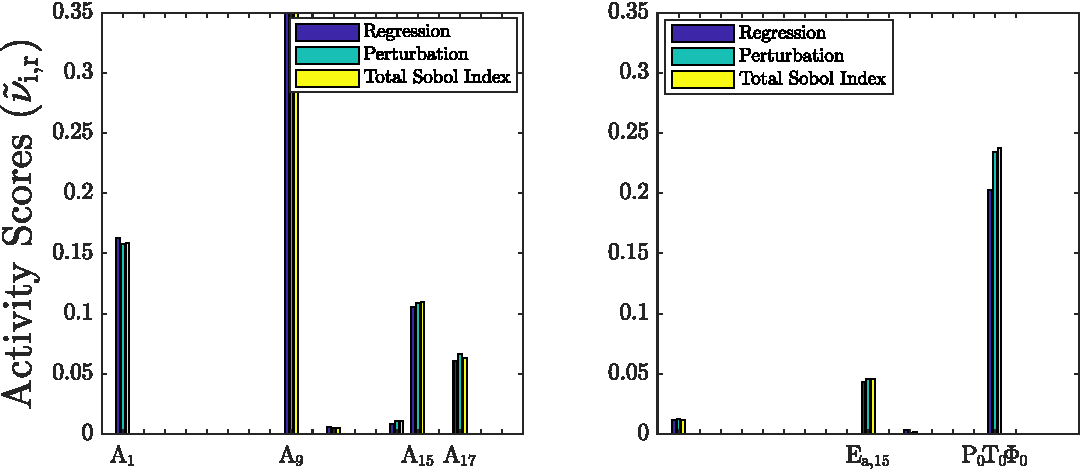
\includegraphics[width=0.8\textwidth]{./Figures/as_36Dp2}
\caption{\rebut{Bar graphs illustrating individual activity scores for the uncertain 
rate parameters and the initial conditions for the H$_2$/O$_2$ reaction.}}
\label{fig:as_36D}
\end{center}
\end{figure}
%
Several useful inferences can be drawn. \rebut{Firstly, the normalized activity scores from the two approaches
and the total-effect Sobol' indices are found to be in close agreement with each other. Secondly, as expected, 
$\tilde{\nu}_{i,r}$ based on perturbation exhibits a better agreement with the total-effect Sobol' indices since
the 1-dimensional
surrogate based on the same approach was used to evaluate the Sobol' indices. This observation demonstrates
that the proposed framework is self-consistent. Thirdly, the variability in the ignition delay is predominantly due
to the uncertainty in $A_1$, $A_9$, and $T_0$ while contributions from the uncertainty in $A_{15}$, $A_{17}$, and
$E_{a,15}$, and $T_0$ are also found to be significant. The remaining rate parameters, initial pressure ($P_0$),
and  stoichiometry ($\Phi_0$) do not seem to impact the ignition delay in their considered intervals. 
Therefore, GSA has helped
identify the important rate parameters i.e. key contributors to the uncertainty, and also demonstrated that among the 
considered uncertain initial conditions, the ignition delay is mainly impacted by the perturbations in the initial 
temperature in the considered interval.}
